% !TEX root = ../main.tex

\chapter{排版格式与规范使用指南}

\section{各级标题与文本排版}

\subsection{正文格式要求}
根据规范要求，正文采用\textbf{小四号宋体}，西文与数字采用 \textbf{Times New Roman}，行距为 1.5 倍行距，段前 0、段后 0，首行缩进 2 字符。

在 \LaTeX{} 中，本模板已通过 \texttt{setup.tex} 自动化配置了相应的行距（\texttt{\textbackslash setstretch\{1.38\}}）与缩进（\texttt{\textbackslash setlength\{\textbackslash parindent\}\{2\textbackslash ccwd\}}）。用户撰写段落时只需正常敲击两次回车分段即可，严禁使用多个全角空格进行手动空格缩进。

\subsection{三级标题示例}
这是一个三级标题示范。根据规范，三级标题采用小四号黑体，首行无缩进，段前 1 行、段后 1 行，1.5 倍行距。其编号格式为“2.1.1 ……”。

\section{图表的绘制与排版规范}

\subsection{表格排版（三线表）}
规范明确要求：\textbf{表的题目在表的上方（五号黑体加粗，居中，段前、段后各空 0.5 行），表的内容采用五号字体，单倍行距}。表格编号建议采用“章节-次序”编号，如“表2-1”。推荐采用学术界通用的标准三线表（\texttt{booktabs} 宏包提供支持）。模板已统一设置图表内容的字号与行距，无需在每个环境中重复设置。

\begin{table}[htbp]
\centering
\caption{机器学习模型在金融反欺诈数据集上的分类性能对比}
\label{tab:model-performance}
\begin{tabularx}{\textwidth}{>{\raggedright\arraybackslash}p{3.6cm}*{4}{>{\centering\arraybackslash}X}}
\toprule
\textbf{模型类别} & \textbf{准确率 (Accuracy)} & \textbf{精确率 (Precision)} & \textbf{召回率 (Recall)} & \textbf{F1 分数} \\
\midrule
Logistic Regression & 82.4\% & 79.1\% & 81.3\% & 0.8018 \\
Support Vector Machine & 87.5\% & 86.2\% & 85.8\% & 0.8599 \\
Random Forest & 91.2\% & 90.7\% & 89.9\% & 0.9030 \\
LightGBM & 94.6\% & 93.8\% & 94.1\% & 0.9395 \\
XGBoost & 95.1\% & 94.5\% & 94.8\% & 0.9465 \\
Deep Neural Network & \textbf{96.8\%} & \textbf{96.2\%} & \textbf{96.5\%} & \textbf{0.9635} \\
\bottomrule
\end{tabularx}
\end{table}

\subsection{插图排版}
规范要求：\textbf{图的题目在图的下方（五号黑体加粗，居中，段前、段后各空 0.5 行），图的内容采用五号字体，单倍行距}。编号采用“图2-1”格式。

\begin{figure}[htbp]
\centering

\includegraphics[width=0.75\textwidth]{figures/swufefull.pdf}
\caption{西南财经大学校名及徽标矢量图示}
\label{fig:swufe-logo-demo}
\end{figure}

\begin{figure}[htbp]
\centering
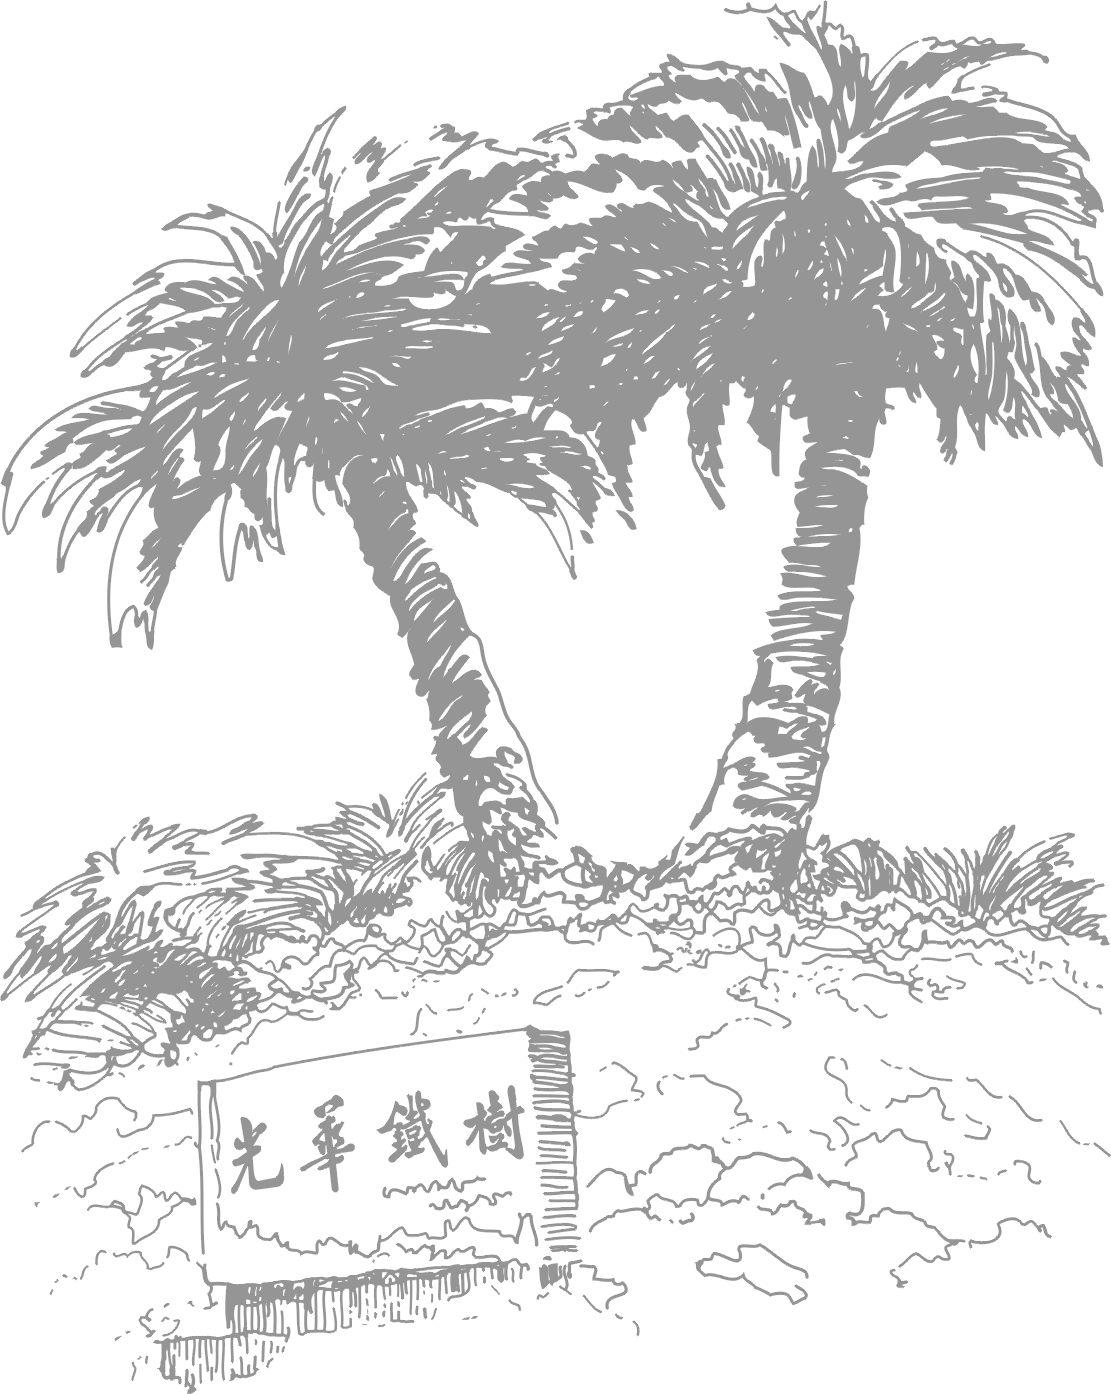
\includegraphics[width=0.45\textwidth]{figures/swufe_cycad.png}
\caption{光华铁树插图示例}
\label{fig:swufe-tree-demo}
\end{figure}

通过 \texttt{\textbackslash ref\{fig:swufe-logo-demo\}} 与 \texttt{\textbackslash ref\{tab:model-performance\}} 可以自动交叉引用，生成的编号分别为图~\ref{fig:swufe-logo-demo} 与表~\ref{tab:model-performance}。

\section{数学公式编写}

规范要求电子稿公式需编号清晰。学术论文中，公式通常采用按章独立连续编号的形式，即形如“(2-1)”。

例如，著名的注意力机制（Attention Mechanism）\cite{Transformer}计算公式如下：
\begin{equation}
\label{eq:attention}
\mathrm{Attention}(Q, K, V) = \mathrm{softmax}\left(\frac{QK^T}{\sqrt{d_k}}\right)V
\end{equation}
其中 $Q, K, V$ 分别表示查询向量（Query）、键向量（Key）和值向量（Value），$d_k$ 为键向量的特征维度。

再如多元高斯分布的概率密度函数公式：
\begin{equation}
\label{eq:multivariate-gaussian}
p(\mathbf{x}; \boldsymbol{\mu}, \boldsymbol{\Sigma}) = \frac{1}{(2\pi)^{d/2}|\boldsymbol{\Sigma}|^{1/2}} \exp\left(-\frac{1}{2}(\mathbf{x}-\boldsymbol{\mu})^T \boldsymbol{\Sigma}^{-1} (\mathbf{x}-\boldsymbol{\mu})\right)
\end{equation}
公式~\eqref{eq:attention} 与公式~\eqref{eq:multivariate-gaussian} 均符合国家标准数学符号规范。

\section{注释与脚注规范}

根据规范要求：“\textbf{毕业论文中有个别名词或情况需要解释时，可加注说明。注释采用脚注，每页独立编号，即每页都从 1 开始编码，编号用 1，2，3……，文中编号用上标}。注释、脚注内容采用小五号宋体或 Times New Roman”。

例如，本文研究中使用了大语言模型\footnote{大语言模型（Large Language Model, LLM）指通常包含数百亿至数千亿参数量、基于大规模文本语料预训练的深度自回归神经网络模型。}，并结合了向量数据库\footnote{向量数据库（Vector Database）是一种专用于高维向量数据的索引检索与相似度计算的专用数据库系统。}进行知识增强。读者可以观察页面底部的脚注，每页从 1 开始重新独立编号，字号为小五号。

\section{算法与代码环境}

\subsection{算法排版}
模板提供了 \texttt{algorithm2e} 宏包支持，可以撰写带行号、规范规整的伪代码：

\begin{algorithm}[H]
\caption{基于动量的随机梯度下降算法 (SGD with Momentum)}
\label{alg:momentum-sgd}
\KwIn{学习率 $\eta$，动量衰减系数 $\gamma \in [0, 1)$，初始模型参数 $\theta_0$}
\KwOut{优化后的模型参数 $\theta^*$}
初始化速度向量 $v_0 \leftarrow 0$\;
\For{$t = 1, 2, \ldots, T$}{
    从训练集中随机采样一个批次样本 $\mathcal{B}_t$\;
    计算小批量样本上的损失函数梯度 $g_t \leftarrow \nabla_\theta \mathcal{L}(\theta_{t-1}; \mathcal{B}_t)$\;
    更新动量速度：$v_t \leftarrow \gamma v_{t-1} + \eta g_t$\;
    更新模型参数：$\theta_t \leftarrow \theta_{t-1} - v_t$\;
    \If{$\|\theta_t - \theta_{t-1}\| < \epsilon$}{
        提前停止迭代\;
        \textbf{break}\;
    }
}
\Return{$\theta_T$}\;
\end{algorithm}

\subsection{代码块排版}
模板内置了 \texttt{codeblock} 环境，支持语法高亮与行号：

\begin{codeblock}[language=Python]
import torch
import torch.nn as nn

class ResidualBlock(nn.Module):
    """ResNet 残差连接模块示例"""
    def __init__(self, channels: int):
        super().__init__()
        self.conv1 = nn.Conv2d(channels, channels, kernel_size=3, padding=1)
        self.bn1 = nn.BatchNorm2d(channels)
        self.relu = nn.ReLU(inplace=True)
        self.conv2 = nn.Conv2d(channels, channels, kernel_size=3, padding=1)
        self.bn2 = nn.BatchNorm2d(channels)

    def forward(self, x: torch.Tensor) -> torch.Tensor:
        residual = x
        out = self.relu(self.bn1(self.conv1(x)))
        out = self.bn2(self.conv2(out))
        out += residual  # 残差跳跃连接
        return self.relu(out)
\end{codeblock}
